%%%%%%%%%%%%%%%%%%%%%%%%%%%%%%%%%%%%%%%%%%%%%%%%%%%%%%%%%%%%%%%%%%%%%%%%%%%%%%%%
%2345678901234567890123456789012345678901234567890123456789012345678901234567890
%        1         2         3         4         5         6         7         8

\documentclass[letterpaper, 10 pt, conference]{ieeeconf}  % Comment this line out
                                                          % if you need a4paper
%\documentclass[a4paper, 10pt, conference]{ieeeconf}      % Use this line for a4
                                                          % paper

\IEEEoverridecommandlockouts                              % This command is only
                                                          % needed if you want to
                                                          % use the \thanks command
\overrideIEEEmargins
% See the \addtolength command later in the file to balance the column lengths
% on the last page of the document



% The following packages can be found on http:\\www.ctan.org
\usepackage{graphicx} % for pdf, bitmapped graphics files
%\usepackage{epsfig} % for postscript graphics files
%\usepackage{mathptmx} % assumes new font selection scheme installed
%\usepackage{times} % assumes new font selection scheme installed
%\usepackage{amsmath} % assumes amsmath package installed
%\usepackage{amssymb}  % assumes amsmath package installed


\title{\LARGE \bf
CS 4758 Robot Learning: Beer Pong Butler
}

%\author{ \parbox{3 in}{\centering Huibert Kwakernaak*
%         \thanks{*Use the $\backslash$thanks command to put information here}\\
%         Faculty of Electrical Engineering, Mathematics and Computer Science\\
%         University of Twente\\
%         7500 AE Enschede, The Netherlands\\
%         {\tt\small h.kwakernaak@autsubmit.com}}
%         \hspace*{ 0.5 in}
%         \parbox{3 in}{ \centering Pradeep Misra**
%         \thanks{**The footnote marks may be inserted manually}\\
%        Department of Electrical Engineering \\
%         Wright State University\\
%         Dayton, OH 45435, USA\\
%         {\tt\small pmisra@cs.wright.edu}}
%}

\author{Kimberly Sheriff - kgs45\\Brian Toth - bdt25}


\begin{document}



\maketitle
\thispagestyle{empty}
\pagestyle{empty}


%%%%%%%%%%%%%%%%%%%%%%%%%%%%%%%%%%%%%%%%%%%%%%%%%%%%%%%%%%%%%%%%%%%%%%%%%%%%%%%%
\begin{abstract}

This paper describes the application of the PR2 robot as a ''Beer Pong Butler", which will identify a ping pong ball in a cup, pick up that cup, and move it to another location. We utilize Hough’s circle detection using OpenCV and an SVM to detect a ball in a cup. We then use motion planning to perform the task given the location of the cup containing a ball.

\end{abstract}


%%%%%%%%%%%%%%%%%%%%%%%%%%%%%%%%%%%%%%%%%%%%%%%%%%%%%%%%%%%%%%%%%%%%%%%%%%%%%%%%
\section{Introduction}

Beer pong, also known as Beirut, is a drinking game typically played at college parties, which involves two teams of two players each throwing ping pong balls across a table with the goal of sinking a ball into a cup of beer at the other end. Figure ~\ref{fig:pongtable}, shows the typical set up for a beer pong game. For our application, we will assume a game played with six cups on each side, which will be empty for our purposes. 

When a ball is successully thrown into a cup, that cup must be removed from the game. The beer pong butler will identify the cup that contains a ball and move that cup away from play.

%\begin{figure}[thpb]
%      \centering
%	  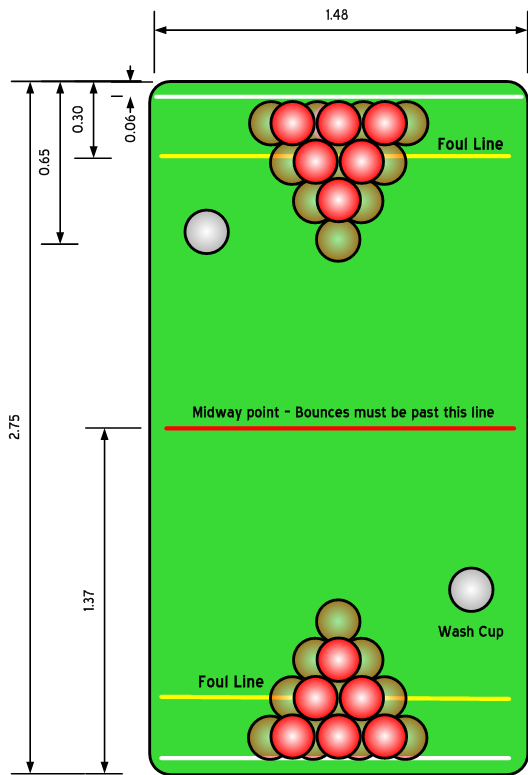
\includegraphics[scale =0.25]{pongtable}
%      \caption{Typical beer pong setup.}
%      \label{fig:pongtable}
%\end{figure}

\subsection{Related Work}

Willow Garage has implemented a PR2 which responds to a "Beer Me" app that allows users to request a beer be brought to them from the fridge. The PR2 navigates to the fridge, uses handle recognition to open the door, and object recognition to determine which beers are in a rack in the fridge. The fridge is modeled using live perception and data from several sources according to a representative from Willow Garage. The PR2  uses motion planning, presumably some type of inverse kinematic solver, to determine the path of the arm to the beer to be picked up.The PR2 is also capable of opening the beer bottle. This algorithm provides the makings of a full service party bot, and our application attempts to provide additional functionality.  

Solem’s Vision Blog explains how to use Hough’s transforms and OpenCV to detect lines and circles on an image of a guage. HoughCircles is a documented function in python which takes as input: the image, the detection method to use, the inverse ratio of the accumulation resolution to the image resolution, minimum distance between the centers of the detected circles, two threshold values, and the minimum and maximum radii. These parameters must be tweaked for different applications.

SVMs are becoming widely used for image classification. David et al. use SVM to genetic syndrome diagnosis which requires image classigication. The results shown in Table 6 of their report shows a comparison between the error rates of the SVM to other machine learning algorithms including 7-nearest neighbor, neural network, and naive bayes. The results show that SVM has the lowest error rate of the compared algorithms. Anthony et al. use SVM for land cover mapping. Their results show high accuracy using both one-versus-one and one-versus-all approaches, and they conclude that the choice between the two methods for image classification is simply personal preference.

From a high level, our approach is to detect the remaining cups, determine which cup has a ball in it, find the X,Y, and Z coordinates of that cup in the base\_link\_frame, and remove that cup from the formation.  This involves learning what a cup looks like and planning motion to a specified point.

\section{Perception}
		
The most complicated and novel part of our project is detecting which cup contains a ball.  Although this sounds simple at first, it rapidly becomes complicated when the possibilities of changing environments, lighting, cups, and viewing angles are considered.

\subsection{Dataset}

To assemble our dataset, we took pictures of formations of cups using the Kinect.  A cup formation is created by placing six cups in a pyramid shapes and then removing between zero and five cups.  To make sure that our data was faithful to the data that would be gathered by the PR2, we placed the Kinect at a height and angle consistent with the PR2's technical documents.  To simulate real-world conditions, we made small adjustments to the height, angle, and position of the Kinect while capturing data, all while varying the lighting conditions.  In some cup formations, one cup holds a ball; in others no cups contain balls.  In total 120 pictures were taken.

50 pictures were reserved for testing and 70 were used for training.  The 70 training examples were sometimes further split into training and validation groups if the particular algorithm being tested required such a split.  Before splitting the data, each picture was manually processed to isolate the cup formation.

\subsubsection{Tabletop Detection}

%TODO: add citations, pictures

In order to segment the tabletop from the objects on the table, we.  Although we were successful in doing so, the resulting pointcloud was not dense enough to actually determine which cup contained the ball.  To solve this, we are currently in the process of overlaying the pointcloud data on the rbg image, with mixed results.

The purpose of detecting the tabletop and removing it from consideration is to isolate the pixels which form the triangle of cups.  Although the image segmentation is not fine-grained enough to detect individual cups, the task of picking out cups from the RBG image is greatly simplified when the image can be cropped to a "blob" which closely follows the cups.


Shown here (clockwise from the right) are the registered pointcloud, the rbg image, and one result of tabletop segmentation projected onto a two dimensional image.  Tabletop segmentation returns significant clusters of points which appear above the tabletop surface.  In this case, one such cluster is the hands and keyboard of the person working at the computer.  The cluster is not yet properly aligned with the RBG image because we have not yet determined which method of coordinate transform is necessary to transform from the Kinect's 3D coordinate frame to its 2D coordinate frame.  Methods attempted include using ROS's tf, projecting the 3D coordinates on to the plane of the observer and rotating that plane, converting the pointcloud to an image directly using ROS's CloudToImage, and simply removing the Z coordinate of each point (most successful, pictured).


\subsubsection{Algorithms}

\subsubsection{Cup Detection}

We considered a number of alternatives for using machine learning to bolster perception.  Although openCV’s Hough Circles do a good job of delimiting cups when properly tuned, as shown in Figure ~\ref{fig:positive}, they can perform erratically when the parameters are a bit off.  Slight changes in environment, lighting, height, or angle can result in incorrect or incomplete labeling of cups as seen in Figure ~\ref{fig:negative}.


Our first idea was to implement a combined HMM and SVM to determine whether we had properly identified the cups.  The problem naturally lends itself to an HMM, because there are a small number of discrete states (configurations of the cups), and the game naturally transitions from one state to another.  Even better, the transition probabilities are certainly not uniform and can be determined experimentally simply by throwing balls into cups.  Although we were very excited about this approach, it was abandoned due to time constraints.  Because each unique configuration would require a custom SVM to be trained, there would have to be 6+6+15+15+20+1+1= 64 different SVMs.  Gathering sufficient data to train and validate this many SVMs would not be practical.

Instead, we are pursuing three different, simpler classifiers which will be compared against our dataset to determine which performs the best.  The ultimate evaluation is the ability to detect if the ball is present and, if it is, where it is located.

The simplest classifier simply looks to determine, for each drawn circle, if that circle represents a valid cup.  Therefore this classifier considers only one cup at a time.  Features include the radius of the circle and the average color of pixels in the circle.  The number of detected cups (and the probability of each circle being a cup) is fed into a simple HMM.  Unlike the HMM mentioned previously, this HMM contains only six states, one for each possible total number of cups.  At each time update, the HMM can either transition to the next state (remove a cup) or keep the same number of cups.  This is used as a sanity check for the circle detector; if the identified number of cups is not equal to the expected number of cups or one fewer than the detector is re-run with different parameters.

The second classifier takes a slightly different approach by considering all of the detected cups at once. Adding the number of cups detected and the number of cups expected as features along with color data for each cup, allows the entire set of circles to be accepted or rejected at once.  This increases the amount of information which can be learned, but has the disadvantage of requiring more guesswork during training (we have to make assumptions about the expected number of cups).

The final classifier goes even further in attempting to consider the entire formation of cups by adding additional features to represent the implicit information in the HMM model.  The first six features represent the “best fit” that the Hough Circle detector can perform given the circles it finds.  Currently the assignment of numbers to cups is done by comparing to the initial 6 cup pyramid.  This makes the assumption that the robot does not significantly move during the course of the game; we are also pursuing an ‘absolute’ model based on coordinates.
    
The information from the “previous state” is incorporated in features 26-31.  Assuming the robot successfully removed a cup in the previous iteration and all of the circles were detected properly, this will match features 1-6 exactly.

The other features are currently experimental attempts to characterize a cup.  This SVM is really doing double-duty; it requires both the detection of the correct number of cups in the correct relative positions and that the circles detected are actually cups.  At present we average the rbg values of the pixels within the cup-circles.\\\\
Features: 
$1 \rightarrow 6$: did the cup detector find cup x. \\
$7 \rightarrow 25$: average rgb values for cups\\
$26 \rightarrow 31$: was the cup there (i.e. should the cup detector have found cup x)\\

Sample feature vector:\\

$1  <1:0 2:1 3:0 4:0 5:0 6:0 7:146.605410924 8:121.33146163 9:135.208269525 .... 26:0 27:1 28:0 29:0 30:0 31:0>$ \\


All of the above use the same method to actually find the ball.  Each identified cup is passed to another SVM which is specifically trained to identify the cup which has the ball.  The features for this SVM are the average color for the cup and the number of orange-like pixels.  This process is separate from the task of actually finding cups, because, until the entire formation is identified, there is little point in searching for the ball.

\subsection{Results}
\newpage
\section{Motion Planning}

The overall goal of the motion planning is to remove the cup, which was determined to contain a ball, from the cup arrangement. To accomplish this goal,  a model of the situation was created in gazebo and inverse kinematics were used to plan the right arm's path. The motion plan assumes that the PR2 is positioned in front of the cup arrangement as shown in Figure~\ref{fig:start} with its arms positioned straight in front of the PR2 body and the grippers pointed upwards at an angle. The motion plan uses only the right arm of the PR2 to complete the goals.

\begin{figure}[thpb]
      \centering
	  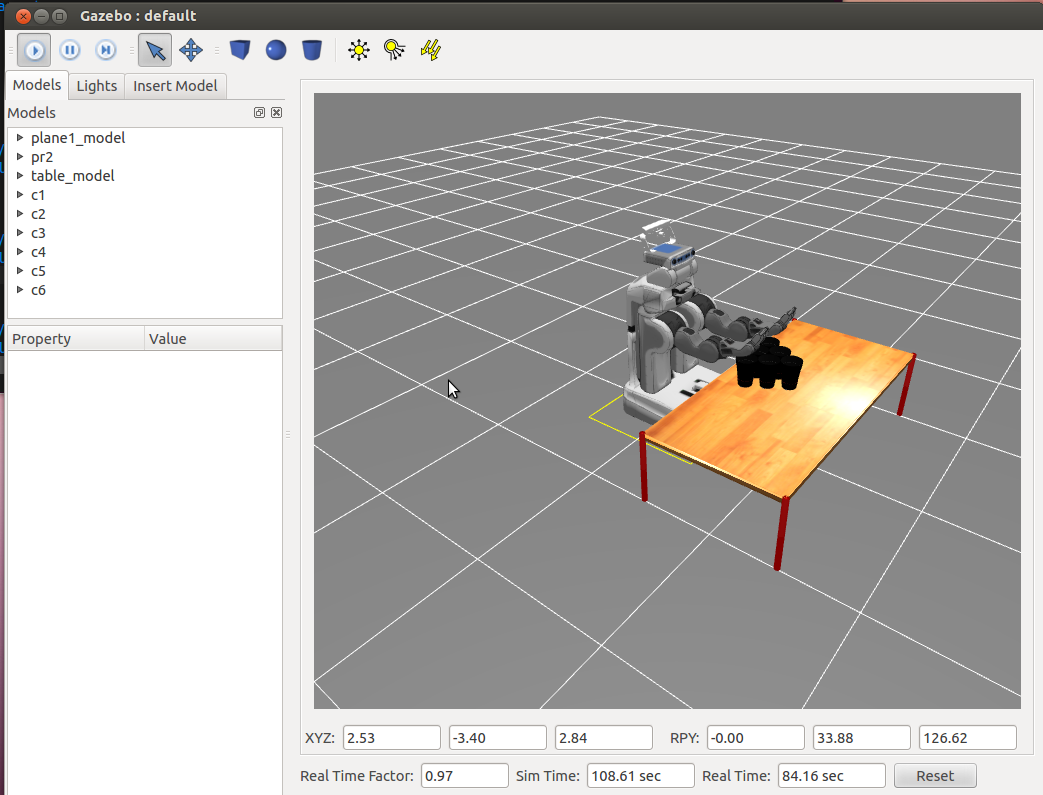
\includegraphics[scale =0.2]{cups_pr2_table}
      \caption{PR2 completing motion task in an empty world.}
      \label{fig:start}
\end{figure}


\subsection{Gazebo Models}
The beer pong scene was modeled in Gazebo using two different object types. The first was the default table object. The second was a plastic cup object to represent the commonly used red plastic SOLO cups used in beer pong. The plastic cup model was sourced from the Google 3D Warehouse. An xml file was created to allow the object to be spawned in the Gazebo world. The cup object had to be scaled in order to fit the scope of the gazebo world. The cup was scaled to 4\% of it's original size to be the approximate size of a real cup with respect to the PR2 and the table in the Gazebo world. Originally the collision map was set to be the same size as the visual cup in gazebo. However, as will be described in the inverse kinematics section below, that size collision map was not ideal. The collision map for the object was shrunk to 3\% of it's original size compared to the visual cup which was scaled to 4\% of it's orginal size. By making the collision map smaller, the gripper was able to move closer to the cup object and inverse kinematics was able to successufly be solved. 

The cup objects were spawned into the gazebo world using the following coordinates as seen in Figure~\ref{fig:cups}:

\begin{description}
\item[Cup 0]  (0.7, 0.15, 0.52)
\item[Cup 1] (0.7, 0.0, 0.52)
\item[Cup 2] (0.7, -0.15, 0.52)
\item[Cup 3] (0.83, 0.075, 0.52)
\item[Cup 4] (0.83, -0.075, 0.52)
\item[Cup 5] (0.96, 0.0, 0.52)
\end{description}

\begin{figure}[thpb]
      \centering
	  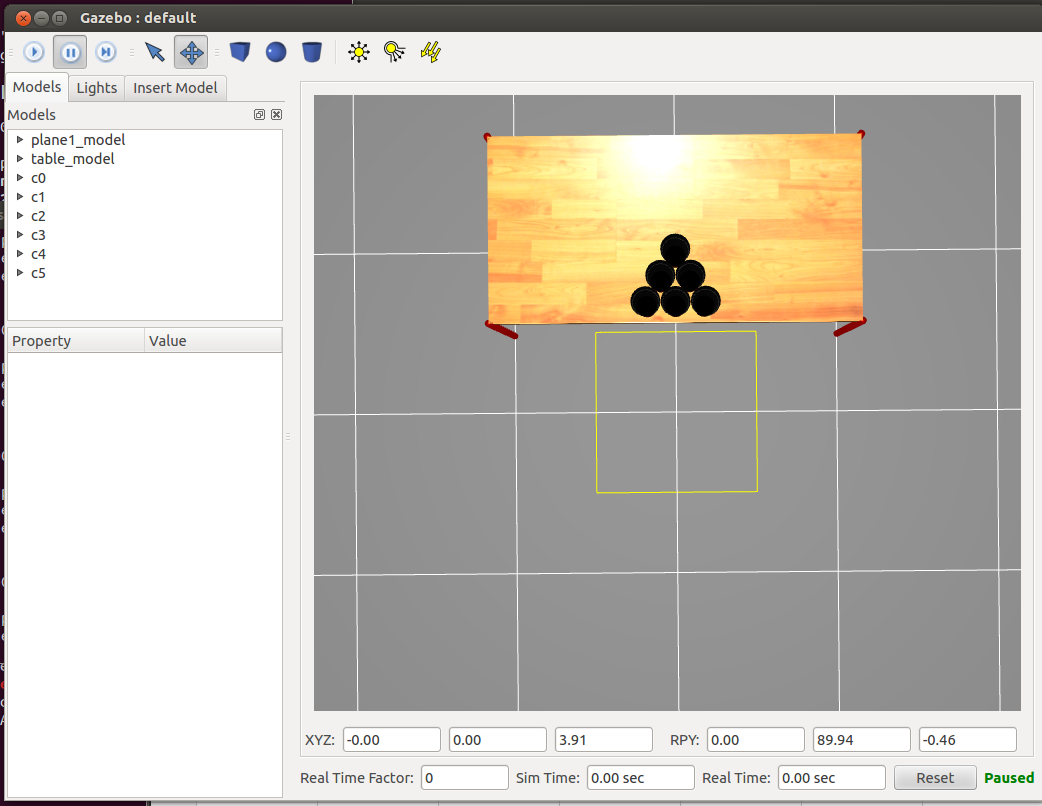
\includegraphics[scale =0.2]{cups}
      \caption{Cup arrangement in gazebo}
      \label{fig:cups}
\end{figure}

These coordinates were chosen because they mimick the real set up of a six cup game, the cup edges do not touch, and the cups do not collide with the table object. By spawning the cups such that they do not touch any other object, the cups are prevented from flying off in a collision.

\subsection{Gripping}
Several gripping techniques were explored in the search for the optimal approach. The two main techniques considered were: gripping one side of the cup and expanding the gripper inside the cup. In the first method, the grip would be positioned such that it is point down vertically at the edge of the cup. The gripper would also be positioned with one side of the gripper on the inside and outside of the plane made by the side of the cup. The gripper would be opened and moved down so that the grippers are on either side of the cup. The gripper would then close and raise the cup away from the arrangement. This method would require the gripper to be positioned fairly accurately above the center of an edge. Furthermore, this method would be difficult to use in a ten cup set up because it would be hard to get to the edges of the middle cup. 

The second method, the gripper would be moved so that it is was pointing veritically over the center of the cup. The gripper would then be lowered into the cup and opened such that it applies a constant pressure to the interior sides of the cup. The gripper would be opened a set distance which would be determined through trial and error using the real PR2. The cup would then be lifted up away from the arrangement with the gripper held open to secure the cup. This method would work for either inner or outer cups as well as cups of different shapes and sizes. Additionally, this method would still work if the gripper was not placed exactly at the center of the cup. The second method was chosen as the final gripping method.

\subsection{Inverse Kinematics}

The overall goal of the inverse kinematics is to move the right arm of the PR2 to complete the following tasks:
\begin{enumerate}
\item move the gripper such that it points down over the center of the cup
\item move the gripper down into the cup 
\item spread the gripper to secure the cup
\item move the gripper up and away to remove the cup from the arrangement
\end{enumerate}

The x,y,z coordinates of the cup we want to move are taken from perception and transformed into the "base\_link" coordinate system from the Kinect coordinate system using the tf package.

The first step was to insure that the PR2 could successfully complete the motion without violating joint limits in an empty world as seen in Figure~\ref{fig:empty}.

\begin{figure}[thpb]
      \centering
	  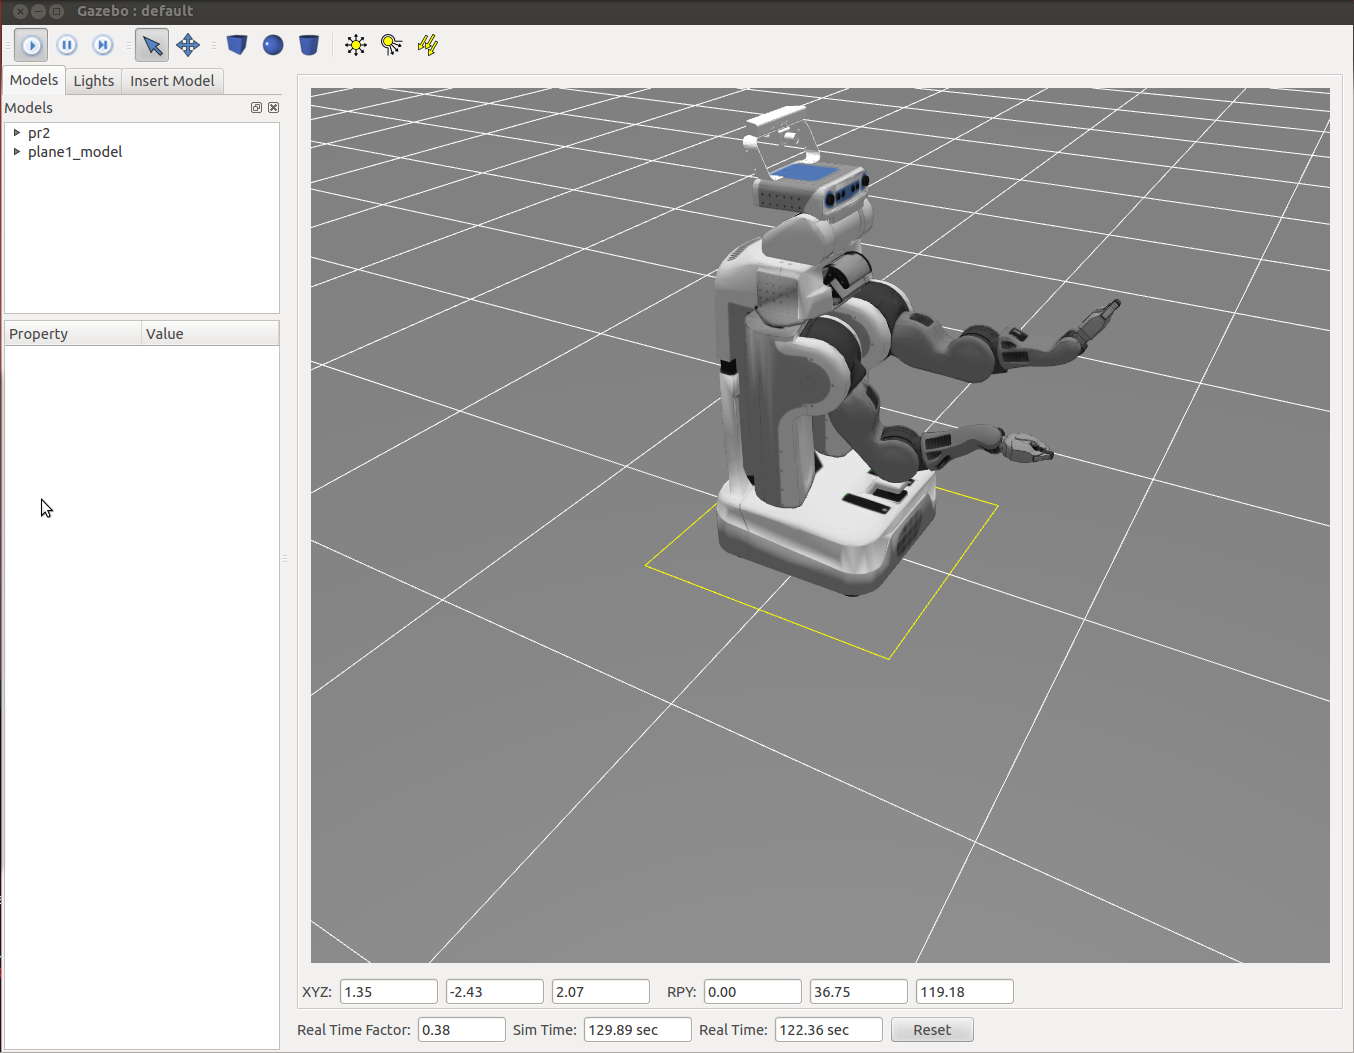
\includegraphics[scale =0.15]{pr2_empty_world}
      \caption{PR2 completing motion task in an empty world.}
      \label{fig:empty}
\end{figure}

After the same movements were confirmed to possible with the table in gazebo, cup 1 was spawned into gazebo and the inverse kinematics was again repeated. However, with the cup in the gazebo, the inverse kinematics failed. The issue was with the collision map of the cup. The collision map was shrunk to be slightly smaller than the visual cup. By shrinking the collision map, the gripper could move closer to the cup and the inverse kinematics were successful. The collision map size was tuned to be small enough to allow inverse kinematics to solve but large enough such that the gripper would not go straight through the visual cup. When the collision map was too small, the arm went straight through the cups and collided with the table as shown in Figure~\ref{fig:dumb}.

\begin{figure}[thpb]
      \centering
	  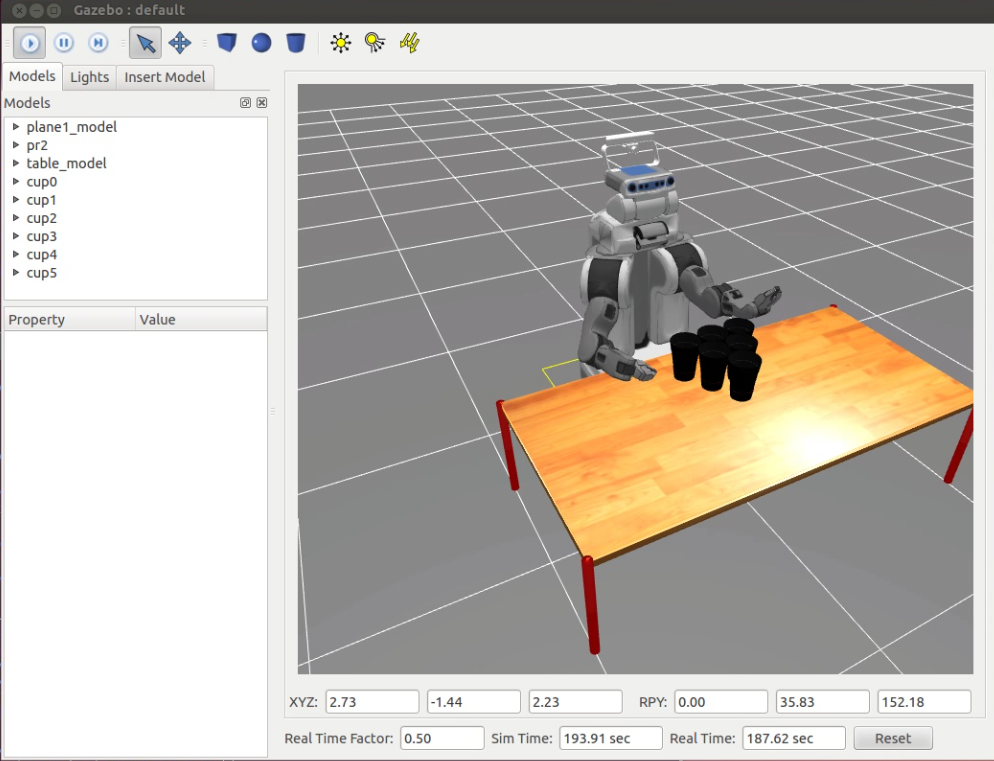
\includegraphics[scale =0.2]{dumb}
      \caption{Effects of too small of a collision map}
      \label{fig:dumb}
\end{figure}

Finally, the motion plan was executed in simulation with the full cup arrangement. We were not able to use the real PR2 because it was not operational. The gripping motion was not able to be performed in gazebo because the physics of gazebo is not ideal. However, we are confident that the designed gripping method we decided on would work if we were able to calibrate it on the real PR2. 

The PR2 first moves the gripper over the cup which will be moved as seen in Figure~\ref{fig:over}. Next the gripper would be spread to secure the cup in the real world scenario.
\begin{figure}[thpb]
      \centering
	  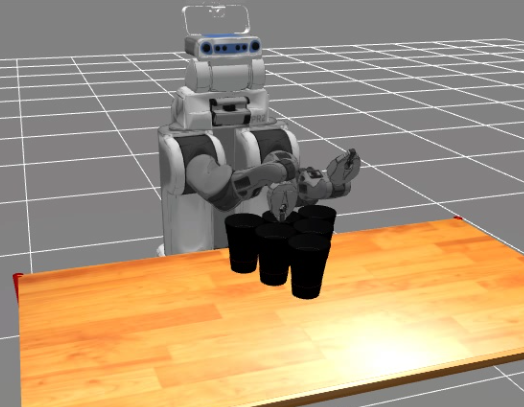
\includegraphics[scale =0.2]{gripper_over_cup}
      \caption{PR2 gripper over cup 1}
      \label{fig:over}
\end{figure}

Finally, the PR2 moves the gripper away from the robot while maintaining control of the cup shown in Figure~\ref{fig:away}.

\begin{figure}[thpb]
      \centering
	  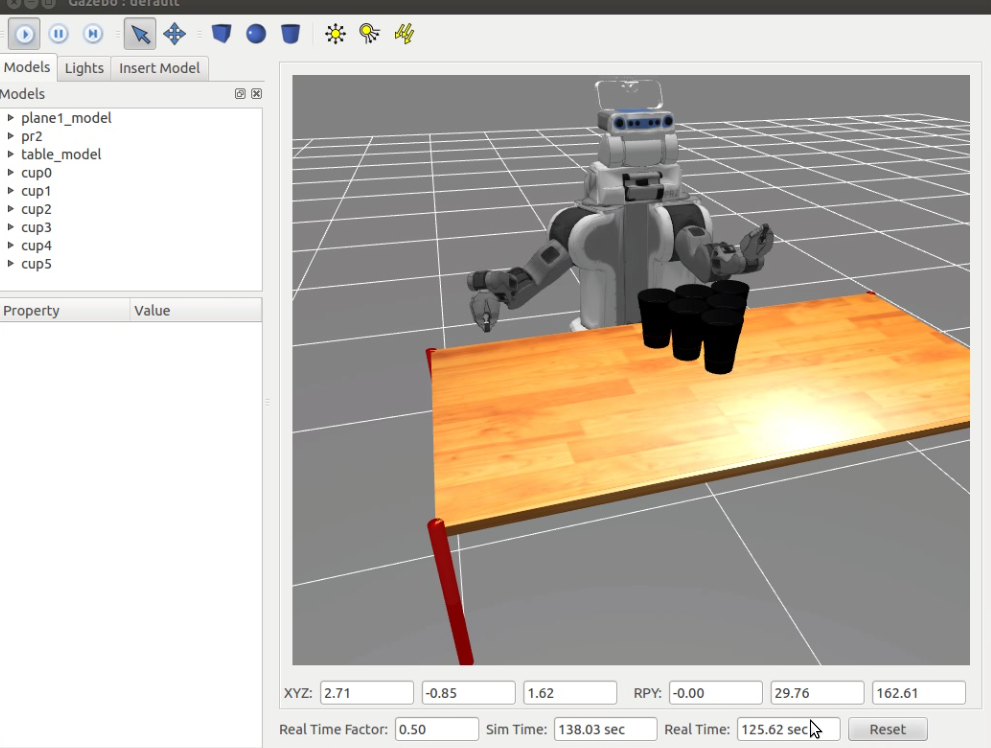
\includegraphics[scale =0.2]{gripper_away}
      \caption{PR2 gripper moved away from arrangement}
      \label{fig:away}
\end{figure}


\subsection{Other Considerations}
We began by working with pick and place, but this algorithm does not work for our application because we are not picking up a stand alone object.




\section{Experiments}

Because our project revolves around detecting which cup has the ball and moving to those XY coordinates

\subsection{Setup}

\subsection{Data}

Our data set is comprised of 51 images taken with the Kinect. We label the cups one to six from left to right starting at the bottom left corner. The images were taken of various configurations of the cups, removing different sets of cups or no cups for each image. The angle and position of the Kinect relative to the cup arrangement was also varied as was the lighting.  A few different red plastic cups were used for the images. 

\subsection{Evaluation Metric}

The ultimate evaluation metric is the ability to detect the ball.  Although many of our methods revolve around detecting cups, this is only an intermediary step.  Thus each image is labeled to indicate the coordinates of the ball (negative coordinates indicate that there is no ball present).  An algorithm succeeds if it selects a point near the ball.

\subsection{Results}

Unfortunately we do not yet have any results for our experiments.  Although we have collected data and are currently implementing multiple learning algorithms, we have not yet run these on the full data set.







\begin{thebibliography}{99}

\bibitem{c1} "Beer Me, Robot." Willow Garage. N.p., n.d. Web. 05 Apr. 2013.
\bibitem{c2} "Feature Detection¶." Feature Detection — OpenCV 2.4.4.0 Documentation. N.p., n.d. Web. 05 Apr. 2013.
\bibitem{c3} http://www.janeriksolem.net/2012/08/reading-gauges-detecting-lines-and.html
\bibitem{c4} Anthony, Gregg, and Tshilidzi. Image Classification Using SVMs: One-against-One Vs One-against-All. Tech. N.p.: n.p., n.d. Print.
\bibitem{c5} David, and Lerner. Support Vector Machine-based Image Classification for Genetic Syndrome Diagnosis. Tech. N.p.: n.p., n.d. Print.







\end{thebibliography}




\end{document}
